\documentclass{atistandalonetask}
\usepackage{atistandard}
\begin{document}

\begin{atiTask}[
	title = Weitere Fragen
]
	\providecommand{\D}{\mathrm{d}}

\begin{atiSubtasks}
	\item Berechnen Sie den Fluss einer Flüssigkeit mit konstanter Geschwindigkeit 
	\[
	\vec{v}=v_{0x}\vec{i}+v_{0y}\vec{j}
	\]
	durch die Kurve $C: x^2+y^2=1$.
	\item Beweisen Sie die folgende Relation im Indexkalkül
	\[\divergence(\vec{a}\times\vec{b})=\vec{b}\curl \vec{a}-\vec{a}\curl\vec{b}
	\]
	\item Berechnen Sie folgende Integrale
	\begin{multicols}{2}
	\begin{atiSubequations}
		\item{\integral{1,5}{2,5}{\delta(x+2)}{x}}
		\item{\integral{0}{2\pi}{\sin x\cdot\delta(x-\pi/2)}{x}}
	    \item{\integral{-\infty}{+\infty}{\ln x\cdot\delta (5(x-1))}{x}}
	    %\item{\integral{0}{\infty}{\frac{e^x}{x^2}\delta(x+1)}{x}}
	    \item{\integral{0}{\infty}{f(x)\cdot\delta(ax^2-b)}{x}}
	\end{atiSubequations}
	\end{multicols}
	\item Gegeben seien die Funktion $f(t)$ und ihre Fouriertransformierte $\hat{f}(k)$. Bestimmen Sie die Fouriertransformierte der Funktion $f(t-a)$.
	\begin{figure}[H]
\centering
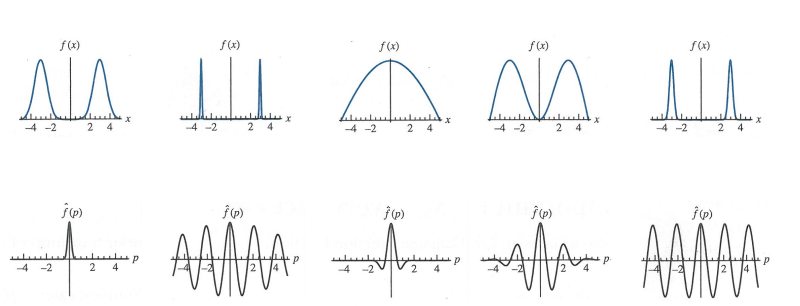
\includegraphics[width=1\linewidth]{./picture-klausurss18}
\end{figure}

	\item Ordnen Sie die Bilder der Funktionen $f(t)$ ihren Fouriertransformierten zu.
	\item \textbf{Zusatz:} Harry und Ron brüten über ihren Arithmantik-Hausaufgaben. \glqq Der Laplace-Operator dieses trimagischen 
	Feldes zeigt nach oben, oder?\grqq{}, fragt Harry. Ron kaut auf seiner Feder herum: \glqq Bei mir zeigt er nach unten\dots\grqq{} Ohne den Blick von ihrem Pergament zu lösen, ruft Hermine: \glqq Ihr liegt beide falsch.\grqq{} Warum?
\end{atiSubtasks}

\end{atiTask}

\end{document}
